\subsection{Results}
The robot sweeps all reachable floor space.
The total traveled path length is 97449.7 m, corresponding to a travel time of 19 hours and 30 minutes.

Figure \ref{floor_sweeping_results} shows part of the offline generated map vs. the traveled path in the same part of the map.

The offline planning part of the code takes 
19.201 seconds to execute
while the robot movement code takes
% 129.698 seconds 
2 minutes and 9.698 seconds 
to complete the coverage.
Timing was measured on a Intel Core i5-3230M CPU with a clock frequency of 3.2GHz.

\begin{figure}[ht]
\centering
  \begin{subfigure}[t]{0.3\textwidth}
    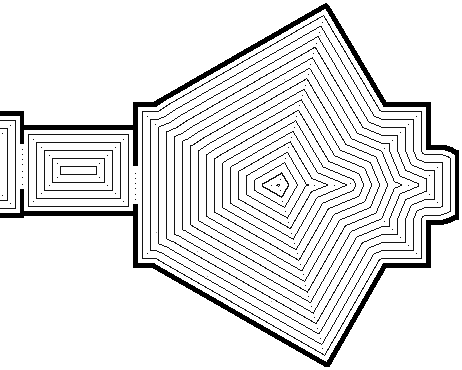
\includegraphics[width = \textwidth]{graphics/floor_sweep_plan}
    \caption{Part of the offline generated map for floor sweeping. The coordinates in \(S_{F}\) are marked.}
    \label{floor_sweep_plan}
  \end{subfigure}
  \begin{subfigure}[t]{0.3\textwidth}
    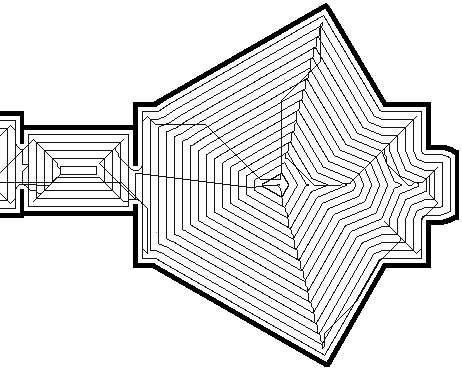
\includegraphics[width = \textwidth]{graphics/floor_sweep_robot}
    \caption{Part of the traveled path in floor sweeping. The coordinates visited are marked.}
    \label{floor_sweep_robot}
  \end{subfigure}
\caption{Floor sweeping planned vs. traveled.}
\label{floor_sweeping_results}
\end{figure}